\documentclass[letterpaper,12pt,fleqn,reqno]{amsart}

\usepackage[margin=1in]{geometry}
\usepackage{tikz}
\usepackage{url}

\newcommand{\R}{\mathbb{R}}
\newcommand{\Q}{\mathbb{Q}}
\newcommand{\uint}{[0,1]}
\newcommand{\usq}{\uint\times\uint}
\newcommand{\pc}{\mathcal{P}}
\newcommand{\pn}{\mathcal{N}}
\newcommand{\po}{\mathcal{O}}
\newcommand{\tick}[1]{\draw (#1,-0.1) -- (#1,0.1)}
\newcommand{\abs}[1]{\left\lvert#1\right\rvert}

\theoremstyle{plain}
\newtheorem{thm}{Theorem}[section]
\newtheorem{lem}[thm]{Lemma}
\newtheorem{defn}[thm]{Definition}
\newtheorem{prop}[thm]{Properties}

\begin{document}

\title{The Peano Curve}

\author{Jeffery Cavallaro}

\address{Department of Mathematics, San Jos\'e State University, San
  Jos\'e, CA 95192-0103}

\email{jeffery.cavallaro@sjsu.edu}

\thanks{\textsc{Math 231A: Real Analysis I}}

\date{\today}

\begin{abstract}
In the late $19^{th}$ century, the field of mathematics was on the verge of a
major explosion. Most of the intuitive problems had already been solved, and
mathematicians were starting to pose questions regarding certain non-intuitive
problems that seemed to shake the mathematical orthodoxy at its core. The trio
of Cantor, Peano, and Hilbert offered the mathematical world methods to wrestle
with these problems, setting the foundations for the practice of mathematical
logic that we take for granted today. One such discovery that epitomizes this
movement was Peano's formulation of a ``space-filling'' curve, and Hilbert's
method for producing such a curve.  Starting with an intuitive isomorphism
between the unit interval and the unit square, one can describe a sequence of
functions that map curves in the unit square. Then, employing some
straightforward (by today's standards) analysis, one arrives at the fairly
non-intuitive result that the sequence of functions converges to one whose map
is surjective on the unit square.
\end{abstract}

\maketitle

\section{Historical Background}

Up until the mid-$19^{th}$ century, mathematics was still limited by the
extreme existentialism of the Hellenistic world view that so enamored the West:
a strong reliance on intuition and an open hostility to the concept of
non-intuitive logic, especially problems involving infinity. But by that time,
most of the ``intuitive'' problems had been solved based on earlier work by
notables such as Euler and Gauss. As a result, mathematicians were starting to
come up with a whole new class of problems whose solutions did not seem to be
solvable using the past intuitive methods.

One popular reaction was to dismiss such problems, usually with a
near-religious zeal, and probably not altogether disconnected from the
nationalism and drive for empire that was sweeping across Europe at the time.
Straight into this fray walked a Russian by the name of Georg Cantor
(1845--1918), whose non-intuitive set theory and formal treatment of infinity
were something completely new and unforeseen. As a result, Cantor was lambasted
by the most vocal in the mathematics community and spent most of his later life
in a sanatorium.

However, Cantor had a soulmate in the person of Guiseppe Peano (1858--1932), a
soft-spoken Italian who attempted to formalize mathematical logic in education
as part of his so-called \emph{Formulario Project}.  Today's analysts may
recall that one of the first things they learned was the Peano axioms on the
natural numbers.  Peano was so well-liked by his students and peers that he
didn't receive the same scorn as Cantor; however, his work was largely ignored
until David Hilbert (1862--1943), a Prussian, started solving many of those
pesky non-intuitive problems using Peano and Cantor's methods.

As the new methods in mathematical logic gained popularity, they were used by
other budding mathematical giants such as Borel and Lebesque in France, and
Riemann and Dedekind in Germany (Gauss's students) to make similar
discoveries. In fact, it was found that many of the so-called non-intuitive
results had concrete applications in the blossoming fields of electrical
engineering and communication theory, born of recent developments in
electricity transmission, the telegraph, and the laying of trans-Atlantic
cables.

One of Peano's discoveries that so epitomizes this movement is his formulation
in 1890 of a continuous, ``space-filling'' curve. Once formulated, it was then
left to Hilbert to come up with a method for generating such a curve.  It is
this formulation and method that we will examine in this paper.

\section{Overview}

The goal is to find a curve $t\mapsto\pc(t)$ with the following properties:
\begin{enumerate}
\item $\pc:\uint\to\usq$.
\item $\pc$ is continuous.
\item $\pc$ is surjective.
\item\label{prop:image} The image under $\pc$ of any $[a,b]\subset\uint$ is a
square $S_{[a,b]}\subset\usq$ such that $m_2(S_{[a,b]})=b-a$.
\end{enumerate}

The gist of property \ref{prop:image} is demonstrated in Figure
\ref{fig:map}.

\begin{figure}[h]
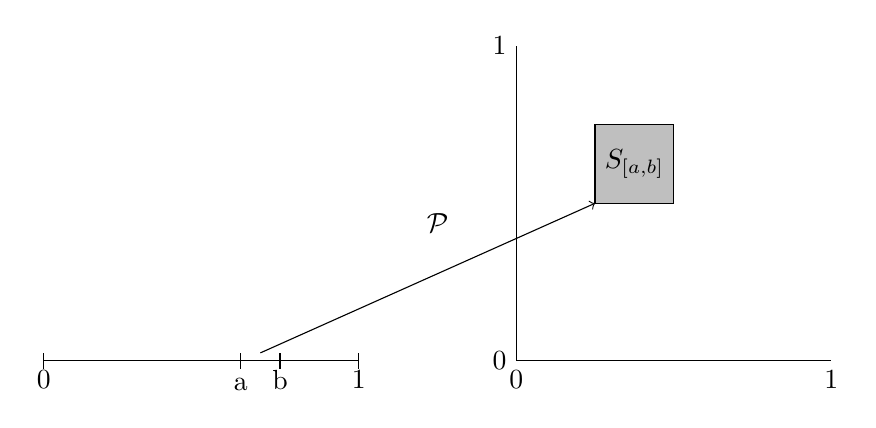
\begin{tikzpicture}
\draw (0,0) -- (4,0);
\tick{0};
\tick{2.5};
\tick{3};
\tick{4};
\node [below] at (0,0) {0};
\node [below] at (2.5,-0.1) {a};
\node [below] at (3,0) {b};
\node [below] at (4,0) {1};

\draw (6,0) -- (10,0);
\draw (6,0) -- (6,4);
\node [below] at (6,0) {0};
\node [left] at (6,0) {0};
\node [below] at (10,0) {1};
\node [left] at (6,4) {1};
\draw [fill=lightgray] (7,2) rectangle (8,3);
\node at (7.5,2.5) {$S_{[a,b]}$};
\draw [->] (2.75, 0.1) -- (7,2);
\node at (5,1.75) {$\pc$};
\end{tikzpicture}
\caption{Demostration of Property \ref{prop:image}}
\label{fig:map}
\end{figure}

Such a mapping is called a \emph{Peano Mapping} and its corresponding curve is
called a \emph{Peano Curve}. Note that this is a parameterized curve from
domain $\R$ to codomain $\R^2$; it is not a mapping \emph{on} $\R$ and thus is
not subject to our normal intuitive notions of a curve in $\R^2$.

The steps in the formulation of $\pc$ are very similar to the construction of a
Cantor set and the terms in the Cantor-Lebesgue function. We start with a
treatment of the domain that continually subdivides each interval into four
equal parts, called \emph{quartic intervals}. Thus, the $n^{th}$ generation
contains $4^n$ almost-disjoint intervals. The codomain receives a similar
treatment, this time into four equal squares, called \emph{dyadic squares}.
Likewise, the $n^{th}$ generation contains $4^n$ almost-disjoint squares.

The matching cardinality between a generation of quartic intervals and its
corresponding generation of dyadic squares invites the definition of a
one-to-one correspondence $\Phi$, referred to as the
\emph{dyadic correspondence}. As we continually refine each quartic interval
and dyadic square, we can see that each collapses to a single point. This
gives rise to an \emph{induced mapping} $\Phi^*$ between the points in the
domain and codomain. Although this mapping is not well-defined on the
boundaries, the locus of the boundaries has measure zero. By eliminating the
boundaries, the induced mapping is well-defined, continuous, and surjective.

To generate the actual curve, we take each generation of dyadic squares and
connect their centers with line segments. We will call the curve for the
$k^{th}$ generation $\pc_k$. Thus, the $\pc_k$ comprise a sequence of uniformly
continuous curves that converge to a continuous curve that is surjective on the
unit square.

Each of these points is explained in detail in the following sections.

\section{Quartic Intervals}
Start with the domain $\uint$. For each generation, subdivide each interval
into four equal parts. This is demonstrated in Figure \ref{fig:quartic}.

\begin{figure}[h]
\begin{tikzpicture}
\node at (-1,0) {\large$I^0$:};
\draw (0,0) -- (8,0);
\tick{0};
\tick{8};
\node [below] at (0,0) {\small0};
\node [below] at (8,0) {\small1};
\end{tikzpicture}

\begin{tikzpicture}
\node at (-1,0) {\large$I^1$:};
\draw (0,0) -- (8,0);
\tick{0};
\tick{2};
\tick{4};
\tick{6};
\tick{8};
\node [below] at (0,0) {\small0};
\node [below] at (2,0) {\small$\frac{1}{4}$};
\node [below] at (4,0) {\small$\frac{2}{4}$};
\node [below] at (6,0) {\small$\frac{3}{4}$};
\node [below] at (8,0) {\small1};
\end{tikzpicture}

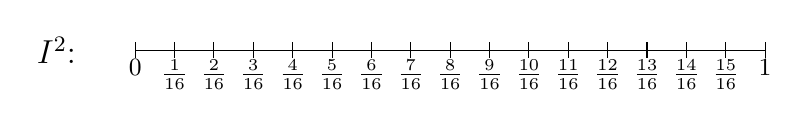
\begin{tikzpicture}
\node at (-1,0) {\large$I^2$:};
\draw (0,0) -- (8,0);
\tick{0};
\tick{0.5};
\tick{1};
\tick{1.5};
\tick{2};
\tick{2.5};
\tick{3};
\tick{3.5};
\tick{4};
\tick{4.5};
\tick{5};
\tick{5.5};
\tick{6};
\tick{6.5};
\tick{7};
\tick{7.5};
\tick{8};
\node [below] at (0,0) {\small$0$};
\node [below] at (0.5,0) {\small$\frac{1}{16}$};
\node [below] at (1,0) {\small$\frac{2}{16}$};
\node [below] at (1.5,0) {\small$\frac{3}{16}$};
\node [below] at (2,0) {\small$\frac{4}{16}$};
\node [below] at (2.5,0) {\small$\frac{5}{16}$};
\node [below] at (3,0) {\small$\frac{6}{16}$};
\node [below] at (3.5,0) {\small$\frac{7}{16}$};
\node [below] at (4,0) {\small$\frac{8}{16}$};
\node [below] at (4.5,0) {\small$\frac{9}{16}$};
\node [below] at (5,0) {\small$\frac{10}{16}$};
\node [below] at (5.5,0) {\small$\frac{11}{16}$};
\node [below] at (6,0) {\small$\frac{12}{16}$};
\node [below] at (6.5,0) {\small$\frac{13}{16}$};
\node [below] at (7,0) {\small$\frac{14}{16}$};
\node [below] at (7.5,0) {\small$\frac{15}{16}$};
\node [below] at (8,0) {\small$1$};
\end{tikzpicture}

\begin{tikzpicture}
\node at (-1,0) {\large$I^n$:};
\draw (0,0) -- (8,0);
\tick{0};
\tick{3};
\tick{4};
\tick{8};
\node [below] at (0,0) {\small0};
\node [below] at (1.5,0) {\small\ldots};
\node [below] at (3,0) {\small$\frac{k}{4^n}$};
\node [below] at (4,0) {\small$\frac{k+1}{4^n}$};
\node [below] at (6,0) {\small\ldots};
\node [below] at (8,0) {\small1};
\end{tikzpicture}
\caption{Generations of Quartic Intervals}
\label{fig:quartic}
\end{figure}

Depending on context, the notation $I^k$ represents either the entire $k^{th}$
generation or a quartic interval from the $k^{th}$ generation. Each generation
has $4^n$ intervals of length (measure):\ $m_1(I^n)=\frac{1}{4^n}$.

We define a refinement of contained intervals as follows:

\begin{defn}
A chain of quartic intervals is a decreasing sequence:
\[I^0\subset I^1\subset I^2\subset\ldots\subset I^k\subset\ldots\]
where $I^k$ is a quartic interval of the $k^{th}$ generation.
\end{defn}

\begin{prop}
Chains of quartic intervals have the following properties:
\begin{enumerate}
\item\label{prop:qiunq} If $(I^k)$ is a chain of quartic intervals then there
exists a unique $t\in\uint$ such that $t\in\bigcap_kI^k$.

\item\label{prop:qiconv} Conversely, given $t\in\uint$, there is a chain $(I^k)$
of quartic intervals such that $t\in\bigcap_kI^k$.

\item\label{prop:qizero} The set of $t$ for which the chain in
(\ref{prop:qiconv}) is not unique is a countable set of measure zero.
\end{enumerate}
\end{prop}

\begin{proof}
Assume that $Q$ is a chain of quartic intervals. Denote the interval in the
$k^{th}$ generation of Q by $[a_k,b_k]$. Then:
\[[0,1]=[a_0,b_0]\supset[a_1,b_1]\supset[a_2,b_2]\supset\cdots\]
or, in general, $[a_k,b_k]\supset[a_{k+1},b_{k+1}]$. So
$a_k\le a_{k+1}\le b_{k+1}\le b_k$ and in particular, 
$a_0\le a_k\le b_k\le b_0$. Thus $(a_k)$ and $(b_k)$ are both monotone, bounded
sequences ($a_k\nearrow$ and $b_k\searrow$) and therefore they both converge.
Let $a=\lim{a_k}=\sup(a_k)$ and $b=\lim{b_k}=\inf(b_k)$. Since
$\forall{k}, a_k\le b_k$, it is the case that $a\le b$. Let $t=a$. So,
$\forall{k},a_k\le t\le b_k$ and:
\[t\in\bigcap_k[a_n,b_n]=\bigcap_kI^k\]
Therefore such a $t$ exists.

Now by way of contradiction, assume that there are two such distinct $t$: $t_1$
and $t_2\in Q$. Let $d=\abs{t_1-t_2}$. There exists a generation $k$ such that
length of one of the intervals in $Q$ is $\frac{1}{4^k}<d$. Assuming that $t_1$
is in this interval, it is clear that $t_2$ is not, resulting in a
contradiction. Therefore $t$ exists and is unique, proving (\ref{prop:qiunq}).

Conversely, given $t\in\uint$, by construction, for each $k$
there is at least one $I^k$ such that $t\in I^k$, proving (\ref{prop:qiconv}).
In fact, non-uniqueness occurs at the boundaries of each interval at the points
$\{\frac{j}{4^k}|0<j<4^k\}$, which is referred to as the set of
\emph{dyadic rationals}. Since the set of dyadic rationals is a countable
subset of $\Q$, it is also countable and has measure zero, thus proving
(\ref{prop:qizero}).
\end{proof}

Similar to the Cantor-Lebesgue function, we can represent each chain of quartic
intervals with a base-4 string of the form $0.a_1a_2\cdots a_k\cdots$ where
each digit selects one of the four sub-intervals in an interval from the
previous generation.  Thus, each $t\in\uint$ can be expressed as:
\begin{equation}
t=\sum_{k=1}^{\infty}\frac{a_k}{4^k}
\label{eqn:quartic}
\end{equation}
which is well-defined except at the dyadic rationals, which correspond to
numbers of the form:
\[0.a_1a_2\cdots a_k0000\cdots=0.a_1a_2\cdots (a_k-1)3333\cdots\]
on the interval boundaries. This corresponds to the fact that each boundary
point is contained in two different chains.

\section{Dyadic Squares}
The codomain gets a similar treatment. Start with the codomain $\usq$. For each
generation, subdivide each square into four equal parts. This is demonstrated
in Figure \ref{fig:dyadic}.

\begin{figure}[h]
\begin{tikzpicture}
\node at (-2,2) {\large$S^0$:};
\draw (0,0) -- (4,0);
\draw (0,4) -- (4,4);
\draw (0,0) -- (0,4);
\draw (4,0) -- (4,4);
\node [below] at (0,0) {\small0};
\node [below] at (4,0) {\small1};
\node [left] at (0,0) {\small0};
\node [left] at (0,4) {\small1};
\end{tikzpicture}
\hspace{0.5in}
\begin{tikzpicture}
\node at (-2,2) {\large$S^1$:};
\draw (0,0) -- (4,0);
\draw (0,2) -- (4,2);
\draw (0,4) -- (4,4);
\draw (0,0) -- (0,4);
\draw (2,0) -- (2,4);
\draw (4,0) -- (4,4);
\node [below] at (0,0) {\small0};
\node [below] at (2,0) {\small$\frac{1}{2}$};
\node [below] at (4,0) {\small1};
\node [left] at (0,0) {\small0};
\node [left] at (0,2) {\small$\frac{1}{2}$};
\node [left] at (0,4) {\small1};
\end{tikzpicture}

\begin{tikzpicture}
\node at (-2,2) {\large$S^2$:};
\draw (0,0) -- (4,0);
\draw (0,1) -- (4,1);
\draw (0,2) -- (4,2);
\draw (0,3) -- (4,3);
\draw (0,4) -- (4,4);
\draw (0,0) -- (0,4);
\draw (1,0) -- (1,4);
\draw (2,0) -- (2,4);
\draw (3,0) -- (3,4);
\draw (4,0) -- (4,4);
\node [below] at (0,0) {\small0};
\node [below] at (1,0) {\small$\frac{1}{4}$};
\node [below] at (2,0) {\small$\frac{2}{4}$};
\node [below] at (3,0) {\small$\frac{3}{4}$};
\node [below] at (4,0) {\small1};
\node [left] at (0,0) {\small0};
\node [left] at (0,1) {\small$\frac{1}{4}$};
\node [left] at (0,2) {\small$\frac{2}{4}$};
\node [left] at (0,3) {\small$\frac{3}{4}$};
\node [left] at (0,4) {\small1};
\end{tikzpicture}
\hspace{0.5in}
\begin{tikzpicture}
\node at (-2,2) {\large$S^n$:};
\draw (0,0) rectangle (4,4);
\draw (1,2) rectangle (2,3);
\draw [dashed] (1,0) -- (1,2);
\draw [dashed] (2,0) -- (2,2);
\draw [dashed] (0,2) -- (1,2);
\draw [dashed] (0,3) -- (1,3);
\node [below] at (0,0) {\small0};
\node [below] at (1,0) {\small$\frac{c}{2^n}$};
\node [below] at (2,0) {\small$\frac{c+1}{2^n}$};
\node [below] at (4,0) {\small1};
\node [left] at (0,0) {\small0};
\node [left] at (0,2) {\small$\frac{r}{2^n}$};
\node [left] at (0,3) {\small$\frac{r+1}{2^n}$};
\node [left] at (0,4) {\small1};
\end{tikzpicture}
\caption{Generations of Dyadic Squares}
\label{fig:dyadic}
\end{figure}

Depending on context, the notation $S^k$ represents either the entire $k^{th}$
generation or a dyadic square from the $k^{th}$ generation. Each generation
has $4^n$ squares ($2^n\times2^n$) of area (measure):\ $m_2(S^n)=\frac{1}{4^n}$
and sides of length $\frac{1}{2^n}$.

We define a refinement of contained intervals as follows:
\begin{defn}
A \emph{chain} of dyadic squares is a decreasing sequence:
\[S^0\subset S^1\subset S^2\subset\ldots\subset S^k\subset\ldots\]
where $S^k$ is a dyadic square of the $k^{th}$ generation.
\end{defn}

Similar to quartic chains:

\begin{prop}
  Dyadic chains have the following properties:
\begin{enumerate}
\item\label{prop:dsunq} If $(S^k)$ is a chain of dyadic squares then there
exists a unique $x\in\usq$ such that $x\in\bigcap_kS^k$.

\item\label{prop:dsconv} Conversely, given $x\in\usq$, there is a chain
$(S^k)$ of dyadic squares such that $x\in\bigcap_kS^k$.

\item\label{prop:dszero} The set of $x$ for which the chain in
(\ref{prop:dsconv}) is not unique is a countable set of measure zero.
\end{enumerate}
\end{prop}

This time, the non-uniqueness occurs at all points $(x_1,x_2)$, where at least
one of the coordinates is a dyadic rational ($4^k=2^{2k}$). The locus of these
points compose the vertical and horizontal line segment boundaries. Since each
vertical segment has measure zero, and since vertical segments occur at a
subset of the dyadic rationals, the vertical segments comprise a set of
measure zero.  Similarly, the horizontal segments comprise a set of measure
zero.  Thus, their union is also a set of measure zero.

Similar to the Cantor-Lebesgue function, we can represent each chain
with a base-4 string of the form $0.b_1b_2\cdots b_k\cdots$ where each digit
selects one of the 4 sub-squares in a square from the previous generation.
Thus, each $x\in\usq$ can be expressed as:
\begin{equation}
x=\sum_{k=1}^{\infty}\frac{\overline{b_k}}{4^k}
\label{eqn:dyadic}
\end{equation}
where
\[\overline{b_k}=\left\{\begin{array}{ll}
(0,0) & b_k=0 \\
(0,1) & b_k=1 \\
(1,0) & b_k=2 \\
(1,1) & b_k=3\end{array}
\right.\]
which is well-defined except along the boundaries.  Note that each non-corner
is contained in two different chains and each corner is contained in four
different chains.

\section{Dyadic Correspondence}

For each generation, $|I^n|=|S^n|$ and within a generation, $m_1(I^n)=m_2(S^n)$.
So, it is possible and desirable to establish a bijection between the quartic
intervals in the domain and the dyadic squares in the co-domain.

\begin{defn}
A dyadic correspondence is a mapping $\Phi$ from collections of quartic
intervals to collections of dyadic squares such that:
\begin{enumerate}
\item $\Phi$ is bijective.
\item $\Phi$ respects generations: $I\in I^k\implies\Phi(I)\in S^k$.
\item $\Phi$ respects inclusion: $I\subset J\implies\Phi(I)\subset\Phi(J)$.
\end{enumerate}
\end{defn}

The trivial correspondence is given by $a_k=b_k$ in equations
(\ref{eqn:quartic}) and (\ref{eqn:dyadic}); however, this results in a
discontinuous mapping of intervals to rectangles. A proper bijection ensures
that adjacent intervals correspond to adjacent squares. The existence of such
a bijection will be proved in section \ref{sec:adj} during the construction of
an actual curve.

Assuming that we have a proper bijection, we can then define the
\emph{induced mapping} $\Phi^*:\uint\to\usq$.

\begin{defn}
Let $\{t\}=\bigcap_{k=1}^{\infty}I^k$ where $(I^k)$ is a chain of quartic
intervals. Then $(\Phi(I^k))$ is a chain of dyadic squares such that
$\bigcap_{k=1}^{\infty}\Phi(I^k)=\{x\}$ and:
\begin{equation}
\Phi^*(t)=x
\end{equation}
\end{defn}

Note that if $I$ is a quartic interval of the $k^{th}$ generation then
$\Phi^*[I]=\Phi(I)$, where $\Phi(I)$ is a dyadic square of the $k^{th}$
generation and: $m_1(I)=m_2(\Phi^*[I])$.

The problem with $\Phi^*$ is that it is not well-defined on the quartic
interval boundary points, since each is representable by two different quartic
chains, resulting in two different dyadic chains. This is addressed in the
following key theorem:

\begin{thm}
Given a dyadic correspondence $\Phi$, there exists sets $Z_1\subset\uint$ and
$Z_2\subset\usq$, both of measure zero, such that:
\begin{enumerate}
\item\label{thm:bij} $\Phi^*:\uint\setminus Z_1\to\usq\setminus Z_2$ is a
bijection.
\item\label{thm:pres} $E\subset\uint$ is measurable iff $\Phi^*[E]\subset\usq$
is measurable.
\item\label{thm:meas} $m_1(E)=m_2(\Phi^*[E])$.
\end{enumerate}
\label{thm:key}
\end{thm}

Before proving this key theorem, the following lemma for quartic intervals is
needed:

\begin{lem}
Let $(f_k)$ be a sequence of base-4 digits as in equation (\ref{eqn:quartic})
and define:
\[E=\left\{t=\sum_{k=1}^{\infty}\frac{a^k}{4^k}\mid
    a_k\ne f_k,\ \mbox{for all sufficiently-large}\ k\right\}\]
Then $m(E)=0$.
\label{lem:quartic}
\end{lem}

\begin{proof}
Assume that $(a_k)$ and $(f_k)$ differ completely starting at digit $r$. Then
the preceding $r-1$ digits of $(a_k)$ select a particular quartic interval, call
it $E_0$. Since $a_r\ne f_r$, one of the four possible sub-intervals in the
next generation is eliminated. Call the remaining three intervals $E_1$.
Continuing this process, we get the following sequence:
\[E_0\supset E_1\supset E_2\supset\ldots\searrow E\]
where $m(E_k)=\frac{3}{4}m(E_{k-1})$ and $m(E_0)<\infty$. Therefore:
\[m(E)=\lim{m(E_0)}=\lim{\left(\frac{3}{4}\right)^n=0}\]
\end{proof}

There is a similar statement for dyadic squares:

\begin{lem}
Let $(f_k)$ be a sequence of base-4 digits as in equation (\ref{eqn:dyadic})
and define:
\[E=\left\{x=\sum_{k=1}^{\infty}\frac{\overline{b^k}}{4^k}\mid
    \overline{b_k}\ne f_k,\ \mbox{for all sufficiently-large}\ k\right\}\]
Then $m(E)=0$.
\label{lem:dyadic}
\end{lem}

With the above lemma, we can now prove part (\ref{thm:bij}) of theorem
\ref{thm:key}.

\begin{proof}
Let $\pn_1$ be the collection of quartic chains for all points $t\in\uint$ that
are not uniquely representable. Also, let $\pn_2$ be the collection of dyadic
chains for all points $x\in\usq$ that are not uniquely representable. By
viewing $\Phi$ more broadly as a bijection between collections of chains,
$\Phi$ is a bijection between $\pn_1\cup\Phi^{-1}(\pn_2)$ and
$\Phi(\pn_1)\cup\pn_2$, as well as between their complements. By letting $Z_1$
be the locus of points in $\pn_1\cup\Phi^{-1}(\pn_2)$ realizable by equation
(\ref{eqn:quartic}), and $Z_2$ be the locus of points in $\Phi(\pn_1)\cup\pn_2$
realizable by equation (\ref{eqn:dyadic}), then the constraint of $\Phi^*$
becomes a well-defined bijection from $\uint\setminus Z_1$ to
$\usq\setminus Z_2$.

To show that $Z_1$ has measure zero, we use lemma \ref{lem:quartic} to select
appropriate $(f_k)$ such that for all chains in $\pn_1$ and $\Phi^{-1}(\pn_2)$,
$a_k\ne f_k$. For example, since each such chain occurs in $\pn_1$ with
trailing digit sequences of all 0's and all 3's, choose $(f_k)$ to be all 1's.
A similar argument using lemma \ref{lem:dyadic} shows that $Z_2$ also has
measure zero.
\end{proof}

Now, with a well-defined version of the bijection $\Phi^*$, parts
(\ref{thm:pres}) and (\ref{thm:meas}) of theorem \ref{thm:key} can be
proved as follows:

\begin{proof}
Assume that $E\subset\uint\setminus Z_1$ is a subset of measure zero. Assume
$\epsilon>0$. $E$ can be covered with a countable set of quartic intervals:
$E=\bigcup_{k}I_k$ such that $\sum_km(I_k)<\epsilon$. Now, since
$\Phi^*[E]\subset\bigcup_k\Phi^*[I_j]$ and because of the fact that
$m_1(I^k)=m_2(S^k)$:
\[m_2(\Phi^*[E])\le\sum_km_2(\Phi^*[I_k])=\sum_km_2(S_k)=\sum_km_1(I_k)<\epsilon\]
Thus, $\Phi^*(E)$ is measurable and has measure zero. Similarly, $(\Phi^*)^{-1}$
maps sets of zero measure in $\usq$ to sets of measure zero in $\uint$.
Therefore, theorem \ref{thm:key} holds for sets of measure zero.

Recall that any open subset of $\uint$ can be written as a countable union of
closed intervals with disjoint interiors. The quartic intervals are such closed
intervals, and so any open set in $\uint$ can be written as a countable union
of quartic intervals. Similarly, any open set in $\usq$ can be written as a
countable union of dyadic squares. Thus, any open set $\po\subset\uint$ can be
written as a countable union of quartic intervals: $\po=\bigcup_kI_k$, the set
$\po\setminus Z_1$ is measurable, and
\[m_2(\Phi^*[\po\setminus Z_1])=\sum_km_2(\Phi^*[I_k])=\sum_km_2(S_k)=
    \sum_km_1(I_k)=m_1(\po\setminus Z_1)\]
Similarly, $(\Phi^*)^{-1}$ maps open sets in $\usq$ to open sets in $\uint$.
Therefore, theorem \ref{thm:key} holds for $G_{\delta}$ sets.

Finally, since every measurable set differs from some $G_{\delta}$ set by a set
of measure zero, theorem \ref{thm:key} holds for all measurable sets $E$.
\end{proof}

\section{Dyadic Correspondence with Adjacency}
\label{sec:adj}

With the Peano mapping properly defined, it is time to turn to Hilbert for the
construction of a Peano curve. Before doing so, we must prove the existence of
a dyadic correspondence that preserves adjacency. To do so, we must first
characterize the possible traversals through the dyadic squares of a given
generation.

Given a dyadic square $S$ in generation $k$, consider its four sub-squares in
generation $k+1$. Assuming we can enter at any square $S_1$, we can always
traverse adjacent squares in a sequence $(S_1, S_2, S_3, S_4)$ and exit at any
edge $\sigma$.  The four possibilities are shown in Figure \ref{fig:trav}.

\begin{figure}[h]
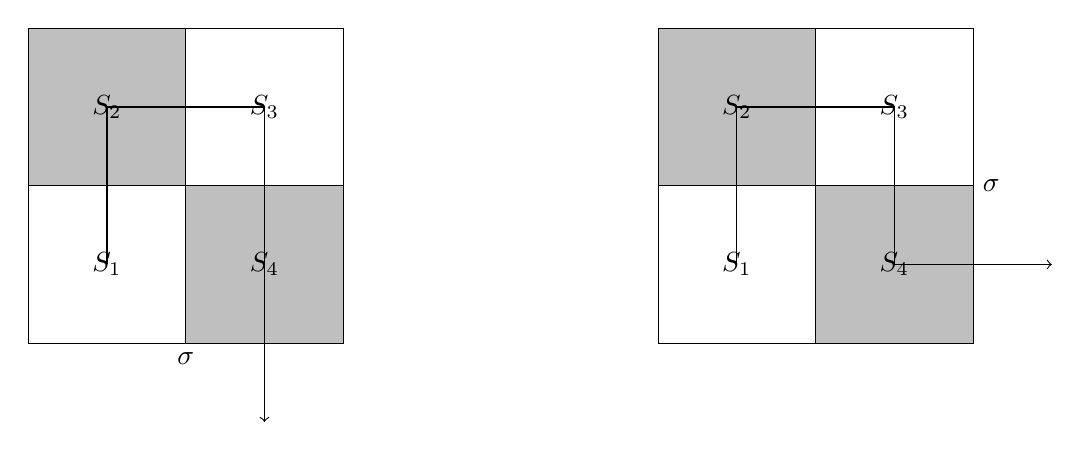
\begin{tikzpicture}
\draw (0,0) rectangle (2,2);
\draw [fill=lightgray] (0,2) rectangle (2,4);
\draw (2,2) rectangle (4,4);
\draw [fill=lightgray] (2,0) rectangle (4,2);
\node at (1,1) {$S_1$};
\node at (1,3) {$S_2$};
\node at (3,3) {$S_3$};
\node at (3,1) {$S_4$};
\node [below] at (2,0) {$\sigma$};
\draw [->] (1,1) -- (1,3) -- (3,3) -- (3,1) -- (3,-1);

\draw (8,0) rectangle (10,2);
\draw [fill=lightgray] (8,2) rectangle (10,4);
\draw (10,2) rectangle (12,4);
\draw [fill=lightgray] (10,0) rectangle (12,2);
\node at (9,1) {$S_1$};
\node at (9,3) {$S_2$};
\node at (11,3) {$S_3$};
\node at (11,1) {$S_4$};
\node [right] at (12,2) {$\sigma$};
\draw [->] (9,1) -- (9,3) -- (11,3) -- (11,1) -- (13,1);
\end{tikzpicture}

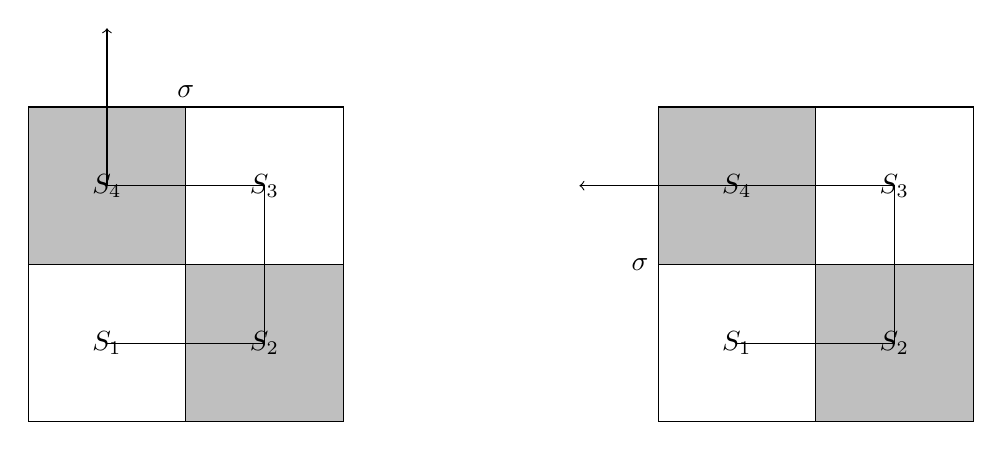
\begin{tikzpicture}
\draw (0,0) rectangle (2,2);
\draw [fill=lightgray] (0,2) rectangle (2,4);
\draw (2,2) rectangle (4,4);
\draw [fill=lightgray] (2,0) rectangle (4,2);
\node at (1,1) {$S_1$};
\node at (1,3) {$S_4$};
\node at (3,3) {$S_3$};
\node at (3,1) {$S_2$};
\node [above] at (2,4) {$\sigma$};
\draw [->] (1,1) -- (3,1) -- (3,3) -- (1,3) -- (1,5);

\draw (8,0) rectangle (10,2);
\draw [fill=lightgray] (8,2) rectangle (10,4);
\draw (10,2) rectangle (12,4);
\draw [fill=lightgray] (10,0) rectangle (12,2);
\node at (9,1) {$S_1$};
\node at (9,3) {$S_4$};
\node at (11,3) {$S_3$};
\node at (11,1) {$S_2$};
\node [left] at (8,2) {$\sigma$};
\draw [->] (9,1) -- (11,1) -- (11,3) -- (9,3) -- (7,3);
\end{tikzpicture}
\caption{Traversal Through a Dyadic Square}
\label{fig:trav}
\end{figure}

Note that each entry square is colored white and each exit square is colored
black. With these possible traversals in hand, we are ready for the next
theorem.

\begin{thm}
There exists a dyadic correspondence $\Phi$ such that:
\begin{enumerate}
\item\label{thm:check} In generation $k$, Let $I_{-}$ be the leftmost interval
and $I_{+}$ be the rightmost interval. $\Phi(I_{-})$ is the lower left square
and $\Phi(I_{+})$ is the lower right square.

\item\label{thm:ind} If $I$ and $J$ are two adjacent intervals in generation
$k$ then $\Phi(I)$ and $\Phi(J)$ are adjacent squares in generation $k$.
\end{enumerate}
\end{thm}

\begin{proof}
For condition (\ref{thm:check}), note that any generation of dyadic squares can
be checkerboarded such that the lower-left square is white (an entry square)
and the lower-right square is black (an exit square). By definitions, we force
$\Phi$ to map the first interval to the lower-left (white) square and the last
interval to the lower-right (black) square.

Condition (\ref{thm:ind}) is proved by induction on generation number $k$. For
the base case let $k=1$:

\begin{center}
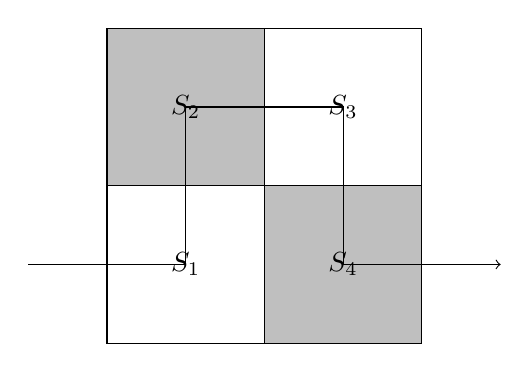
\begin{tikzpicture}
\draw (0,0) rectangle (2,2);
\draw [fill=lightgray] (0,2) rectangle (2,4);
\draw (2,2) rectangle (4,4);
\draw [fill=lightgray] (2,0) rectangle (4,2);
\node at (1,1) {$S_1$};
\node at (1,3) {$S_2$};
\node at (3,3) {$S_3$};
\node at (3,1) {$S_4$};
\draw [->] (-1,1) -- (1,1) -- (1,3) -- (3,3) -- (3,1) -- (5,1);
\end{tikzpicture}
\end{center}

Assume $\Phi$ has been defined for all generations $\le k$ and consider
generation $k+1$. Assume that $S_j$ is a square from generation $k$ that has
been divided into squares $S_{j,1}, S_{j,2}, S_{j,3}, S_{j,4}$ in generation $k+1$.
Square $S_j$ is entered from adjacent square $S_{j-1}$ by a traversal from a
black square in $S_{j-1}$ to a white square in $S_j$. Let $\sigma$ be the edge
between $S_j$ and $S_{j+1}$. Traverse $S_j$ using one of the four valid
traversals to reach $S_{j+1}$.

By the inductive assumption, $S_{4^k}$ is in the lower-right corner, and must be
entered from adjacent square $S_{4^k-1}$ from either the top or left. Since the
lower-left square in generation $k+1$ is an exit square, it must be black.
Since we must enter $S_{4^k}$ on a white square, only one of the following two
cases is possible:

\bigskip

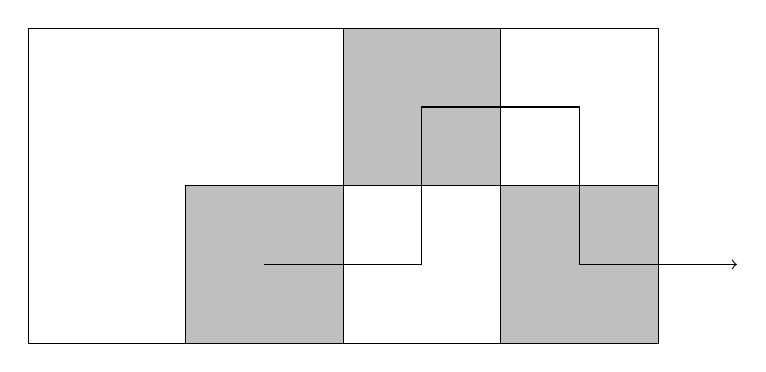
\begin{tikzpicture}
\draw (0,0) rectangle (4,4);
\draw [fill=lightgray] (2,0) rectangle (4,2);
\draw (4,0) rectangle (6,2);
\draw [fill=lightgray] (4,2) rectangle (6,4);
\draw (6,2) rectangle (8,4);
\draw [fill=lightgray] (6,0) rectangle (8,2);
\draw [->] (3,1) -- (5,1) -- (5,3) -- (7,3) -- (7,1) -- (9,1);
\end{tikzpicture}

\bigskip

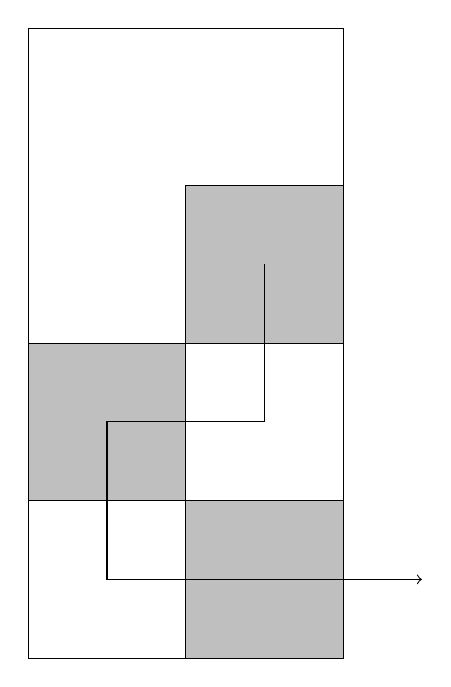
\begin{tikzpicture}
\draw (0,0) rectangle (2,2);
\draw [fill=lightgray] (0,2) rectangle (2,4);
\draw (2,2) rectangle (4,4);
\draw [fill=lightgray] (2,0) rectangle (4,2);
\draw (0,4) rectangle (4,8);
\draw [fill=lightgray] (2,4) rectangle (4,6);
\draw [->] (3,5) -- (3,3) -- (1,3) -- (1,1) -- (3,1) -- (5,1);
\end{tikzpicture}

\bigskip

Therefore, $\Phi$ is properly defined for generation $k+1$.
\end{proof}

\section{The Curve}

With a proper dyadic correspondence $\Phi$ that preserves adjacency, we are now
ready to construct the curve. For generation $k$, let $t_j$ be the center of
the $j^{th}$ quartic interval:
\[t_j=\frac{j-\frac{1}{2}}{4^k}, 1\le j\le4^k\]
and let $x_j$ be the center of the $j^{th}$ dyadic square per the ordering
imposed by $\Phi$. Define:
\[\pc(t)=\begin{cases}
x_j & t=t_j \\
(0,\frac{1}{2^{k+1}})=x_0 & t=t_0=0 \\
(1,\frac{1}{2^{k+1}})=x_{4^k+1} & t=t_{4^k+1}=1 \\
\end{cases}\]

For each sub-interval $[t_j,t_{j+1}],0\le j\le1$, define a linear mapping to
the vertical or horizontal line segment joining the corresponding $x_j$ and
$x_{j+1}$. An example construction for $\pc_2$ is shown in Figure \ref{fig:line}.

\begin{figure}[h]
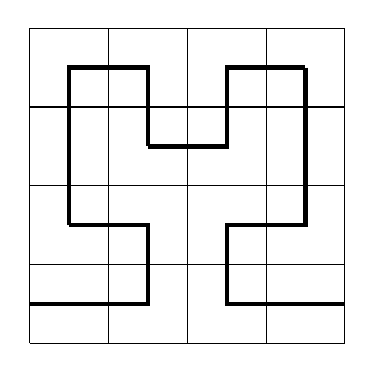
\begin{tikzpicture}
\draw (0,0) -- (4,0);
\draw (0,1) -- (4,1);
\draw (0,2) -- (4,2);
\draw (0,3) -- (4,3);
\draw (0,4) -- (4,4);
\draw (0,0) -- (0,4);
\draw (1,0) -- (1,4);
\draw (2,0) -- (2,4);
\draw (3,0) -- (3,4);
\draw (4,0) -- (4,4);
\draw [ultra thick] (0,1/2) -- (3/2,1/2) -- (3/2,3/2) -- (1/2,3/2);
\draw [ultra thick] (1/2,3/2) -- (1/2,7/2) -- (3/2,7/2) -- (3/2,5/2);
\draw [ultra thick] (1/2,3/2) -- (1/2,7/2) -- (3/2,7/2) -- (3/2,5/2);
\draw [ultra thick] (3/2,5/2) -- (5/2,5/2) -- (5/2,7/2) -- (7/2,7/2);
\draw [ultra thick] (7/2,7/2) -- (7/2,3/2) -- (5/2,3/2) -- (5/2,1/2) -- (4,1/2);
\end{tikzpicture}
\caption{A Construction for $\pc_2$}
\label{fig:line}
\end{figure}

\begin{thm}
$P_k(t)$ is continuous.
\end{thm}

\begin{proof}
Assume $\epsilon>0$ and let $\delta=\frac{\epsilon}{2^k}$. Note that the
worst-case $\abs{\pc(t_1)-\pc(t_2)}$ occurs along adjacent all vertical or
all horizontal line segments.  In such a case,
$P_k'(t)=\frac{\frac{1}{2^k}}{\frac{1}{4^k}}=2^k$, and thus
$\abs{\pc(t_1)-\pc(t_2)}\le2^k\abs{t_1-t_2}<2^k\delta=
    2^k\left(\frac{\epsilon}{2^k}\right)=\epsilon$
\end{proof}

\begin{thm}
$\pc$ exists, is continuous, and surjective.
\end{thm}

\begin{proof}
Note that since $\pc_{k+1}(t)$ and $\pc_k(t)$ are in the same dyadic square
in generation $k$:
\[\abs{\pc_{k+1}(t)-\pc_k(t)}\le\frac{\sqrt{2}}{2^k}\]
and thus the limit:
\[\pc=\lim{\pc_k}=\pc_1+\sum_{j=1}^{\infty}\left(\pc_{k+1}-\pc_k\right)\]
exists. Furthermore, $\pc$ is continuous since the $\pc_k$ are uniformly
continuous. Moveover, since $\pc_k$ visits every dyadic square in generation
$k$, $\pc$ is dense in $\usq$.  Since $\pc$ is both continuous and dense, it is
also surjective.
\end{proof}

The final step is to prove that $\pc=\Phi^*$.

\begin{thm}
$\Phi^*(t)=\pc(t)$.
\end{thm}

\begin{proof}
Assume $t\in\uint$.
\[\Phi^*(t)=\Phi^*\left(\bigcap_kI_k\right)=\bigcap_k\Phi(I_k)=
    \bigcap_kS_k=x=\pc(t)\]
\end{proof}

\nocite{*}
\bibliographystyle{amsplain} 
\bibliography{ref}    

\end{document}
